\subsubsection*{A. Appetizing problem}
\problemauthor{Баев А.Ж.}

Ответ:
$$
4T+D+\left[\frac{N_1}{100}\right]+\left[\frac{N_2}{100}\right]-2. 
$$
Асимптотика --- $O(1)$.


\subsubsection*{B. Bekarys' problem}
\problemauthor{Абдикалыков А.К.}

Если $n<20$, то найти $n!$ явно и выделить его четвёртую цифру справа. Если $n\geqslant 20$, то ничего считать не надо --- ответ будет заведомо 0.\\
Асимптотика --- $O(1)$.

\subsubsection*{С. Car showroom problem}
\problemauthor{Абдикалыков А.К.}

Найти количество строк из строчных латинских букв длины $n$, не содержащих подстроки <<aa>>. Нетрудно вывести (рассматривая, например, отдельно строки, оканчивающиеся на 'a' и оканчивающиеся не на 'a') рекуррентную формулу
$$
a_n = (p-1)(a_{n-1}+a_{n-2}).
$$
Здесь $a_n$ --- ответ на задачу при заданном $n$. Чтобы его найти, надо использовать эту формулу, положив $a_0=1$, $a_1=26$.\\
Асимптотика --- $O(n)$.
 
\subsubsection*{D. Dice problem}
\problemauthor{Баев А.Ж.}

Определить, через какое минимальное число перекатываний по доске можно изменить состояние кубика с {\tt (1, 1, RED\_DOWN)} на {\tt (1, 1, RED\_UP)}. Используем обход в ширину для специального графа: его вершинами будут тройки {\tt (i, j, state)}, где $(i, j)$ --- позиция кубика, $state$ --- одно из шести его положений: {\tt RED\_UP, RED\_DOWN, RED\_LEFT, RED\_RIGHT, RED\_FRONT, RED\_BACK}. 

То есть необходимо для каждого из 6 положений красной грани определить положение после каждого из 4 видов перекативаний: итого 24 перехода. Например, при перекатывании вниз из положения {\tt (i, j, RED\_UP)}, получаем положение {\tt (i + 1, j, RED\_FRONT)}. Они будут соединены ребром. При этом надо учитывать, что некоторые клетки недостижимы.

Асимптотика --- $O(mn)$.


\subsubsection*{E. Easy problem}
\problemauthor{Баев А.Ж.}

Найти количество таких пар $(i, j)$, что $1\leqslant i < j \leqslant n$ и $L \leqslant \dfrac{a_i+a_j}{2}\leqslant R$. Отсортируем числа $a_1, \hdots, a_n$, затем для каждого $a_i$ с помощью бинарного поиска найдём минимальный индекс $p_i$ такой, что $a_{p_i} \geqslant 2L - a_i$ и максимальный индекс $q_i$ такой, что $a_{q_i} \leqslant 2R - a_i$. Просуммировав все $(q_i-p_i+1)$, получим ответ.\\
Асимптотика --- $O(n\cdot log n)$. 

\subsubsection*{F. Flat problem}
\problemauthor{Баев А.Ж.}
 
Определить, какое максимальное количество стен можно поставить в фигуре из клеток, чтобы она оставалась связной.

\begin{center}
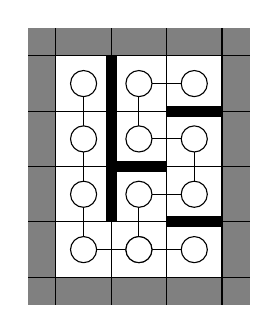
\begin{tikzpicture}[x=20,y=20]
\fill[color=gray](0.5,0.5) rectangle (4.5,5.5);
\fill[color=white](1,1) rectangle (4,5);
\draw[step=1] (0.5,0.5) grid (4.5, 5.5);

\draw[line width=4pt] (2,2) -- (2, 5);
\draw[line width=4pt] (3,3) -- (2, 3);
\draw[line width=4pt] (3,2) -- (4, 2);
\draw[line width=4pt] (3,4) -- (4, 4);

\draw 
(1.5, 4.5) node [shape=circle, draw, fill = white]{} -- (1.5, 3.5) node [shape=circle, draw, fill = white]{} -- (1.5, 2.5) node [shape=circle, draw, fill = white]{} -- (1.5, 1.5) node [shape=circle, draw, fill = white]{} -- (2.5, 1.5) node [shape=circle, draw, fill = white]{} --
(3.5, 1.5) node [shape=circle, draw, fill = white]{};
\draw
(2.5, 1.5) node [shape=circle, draw, fill = white]{} --
(2.5, 2.5) node [shape=circle, draw, fill = white]{} --
(3.5, 2.5) node [shape=circle, draw, fill = white]{} --
(3.5, 3.5) node [shape=circle, draw, fill = white]{} --
(2.5, 3.5) node [shape=circle, draw, fill = white]{} --
(2.5, 4.5) node [shape=circle, draw, fill = white]{} --
(3.5, 4.5) node [shape=circle, draw, fill = white]{};
\end{tikzpicture}
\end{center}

Сопоставим полученной клеточной области граф, вершины которого соответствуют клеткам, а две вершины соединены ребром только в том случае, если соответствующие клетки имеют общую сторону. Нетрудно видеть, что теперь задача сводится к следующему вопросу: какое максимальное количество рёбер можно удалить из графа, чтобы он оставался связным? Ясно, что останется дерево, то есть ответом будет число $E - V + 1$. Ограничения позволяют посчитать количество всех свободных клеток и количество соседних пар наивно на булевой таблице размера $2001 \times 2001$.\\
Асимптотика --- $O(L^2)$.

\newpage

\subsubsection*{G. Golden problem}
\problemauthor{Баев А.Ж.}

Для каждого запроса определить, сколько не палиндромов, дающих в квадрате палиндром, находится на сегменте $[L, R]$. Таких чисел до $10^9$ всего 24:
\begin{center}
\begin{tabular}{lll}
1 : 26   &
2 : 264  &
3 : 307  \\
4 : 836  &
5 : 2285  &
6 : 2636  \\
7 : 22865  &
8 : 24846  &
9 : 30693  \\
10 : 798644  &
11 : 1042151  &
12 : 1109111  \\
13 : 1270869  &
14 : 2012748  &
15 : 2294675  \\
16 : 3069307  &
17 : 11129361  &
18 : 12028229  \\
19 : 12866669  &
20 : 30001253  &
21 : 64030648  \\
22 : 110091011  &
23 : 111091111  &
24 : 306930693  \\
\end{tabular}
\end{center}

Достаточно было их предпросчитать во вспомогательной программе, а затем перебирать для каждого запроса. Простейший наивный генератор вычисляет все 24 числа за 3 минуты.\\
Асимптотика --- $O(M)$.


\subsubsection*{H. Honey cake problem}
\problemauthor{Баев А.Ж.}

Определить, чередуются ли в данном многоугольнике выпуклые углы с невыпуклыми. Нужно было вычислить все ориентированные площади вида $S_i = S_{A_iA_{i+1}A_{i+2}}$. Многоугольник будет удовлетворять условию, только если $S_i$ чередуются знаками и количество вершин чётное.\\
Асимптотика --- $O(M)$.


\subsubsection*{I. Is that even a problem?}
\problemauthor{Абдикалыков А.К.}

Подсказка: мама --- первое слово у детей, абырвалг --- первое слово Шарикова, Поехали! --- первое слово Гагарина перед полетом в космос.

Поставив вместе все первые слова из текстов остальных задач, вы получите выражение
\begin{center}
Дважды А да куб В плюс квадрат С,
\end{center}
то есть, ответ
$$
ans = 2A+B^3+C^2.
$$
Асимптотика --- $O(1)$.